\chapter{Anhang}



\section{Zeitplan}
\label{attachment:zeitplan}
\begin{figure}[H]
    \caption{Zeitplan (eigene Darstellung)}
    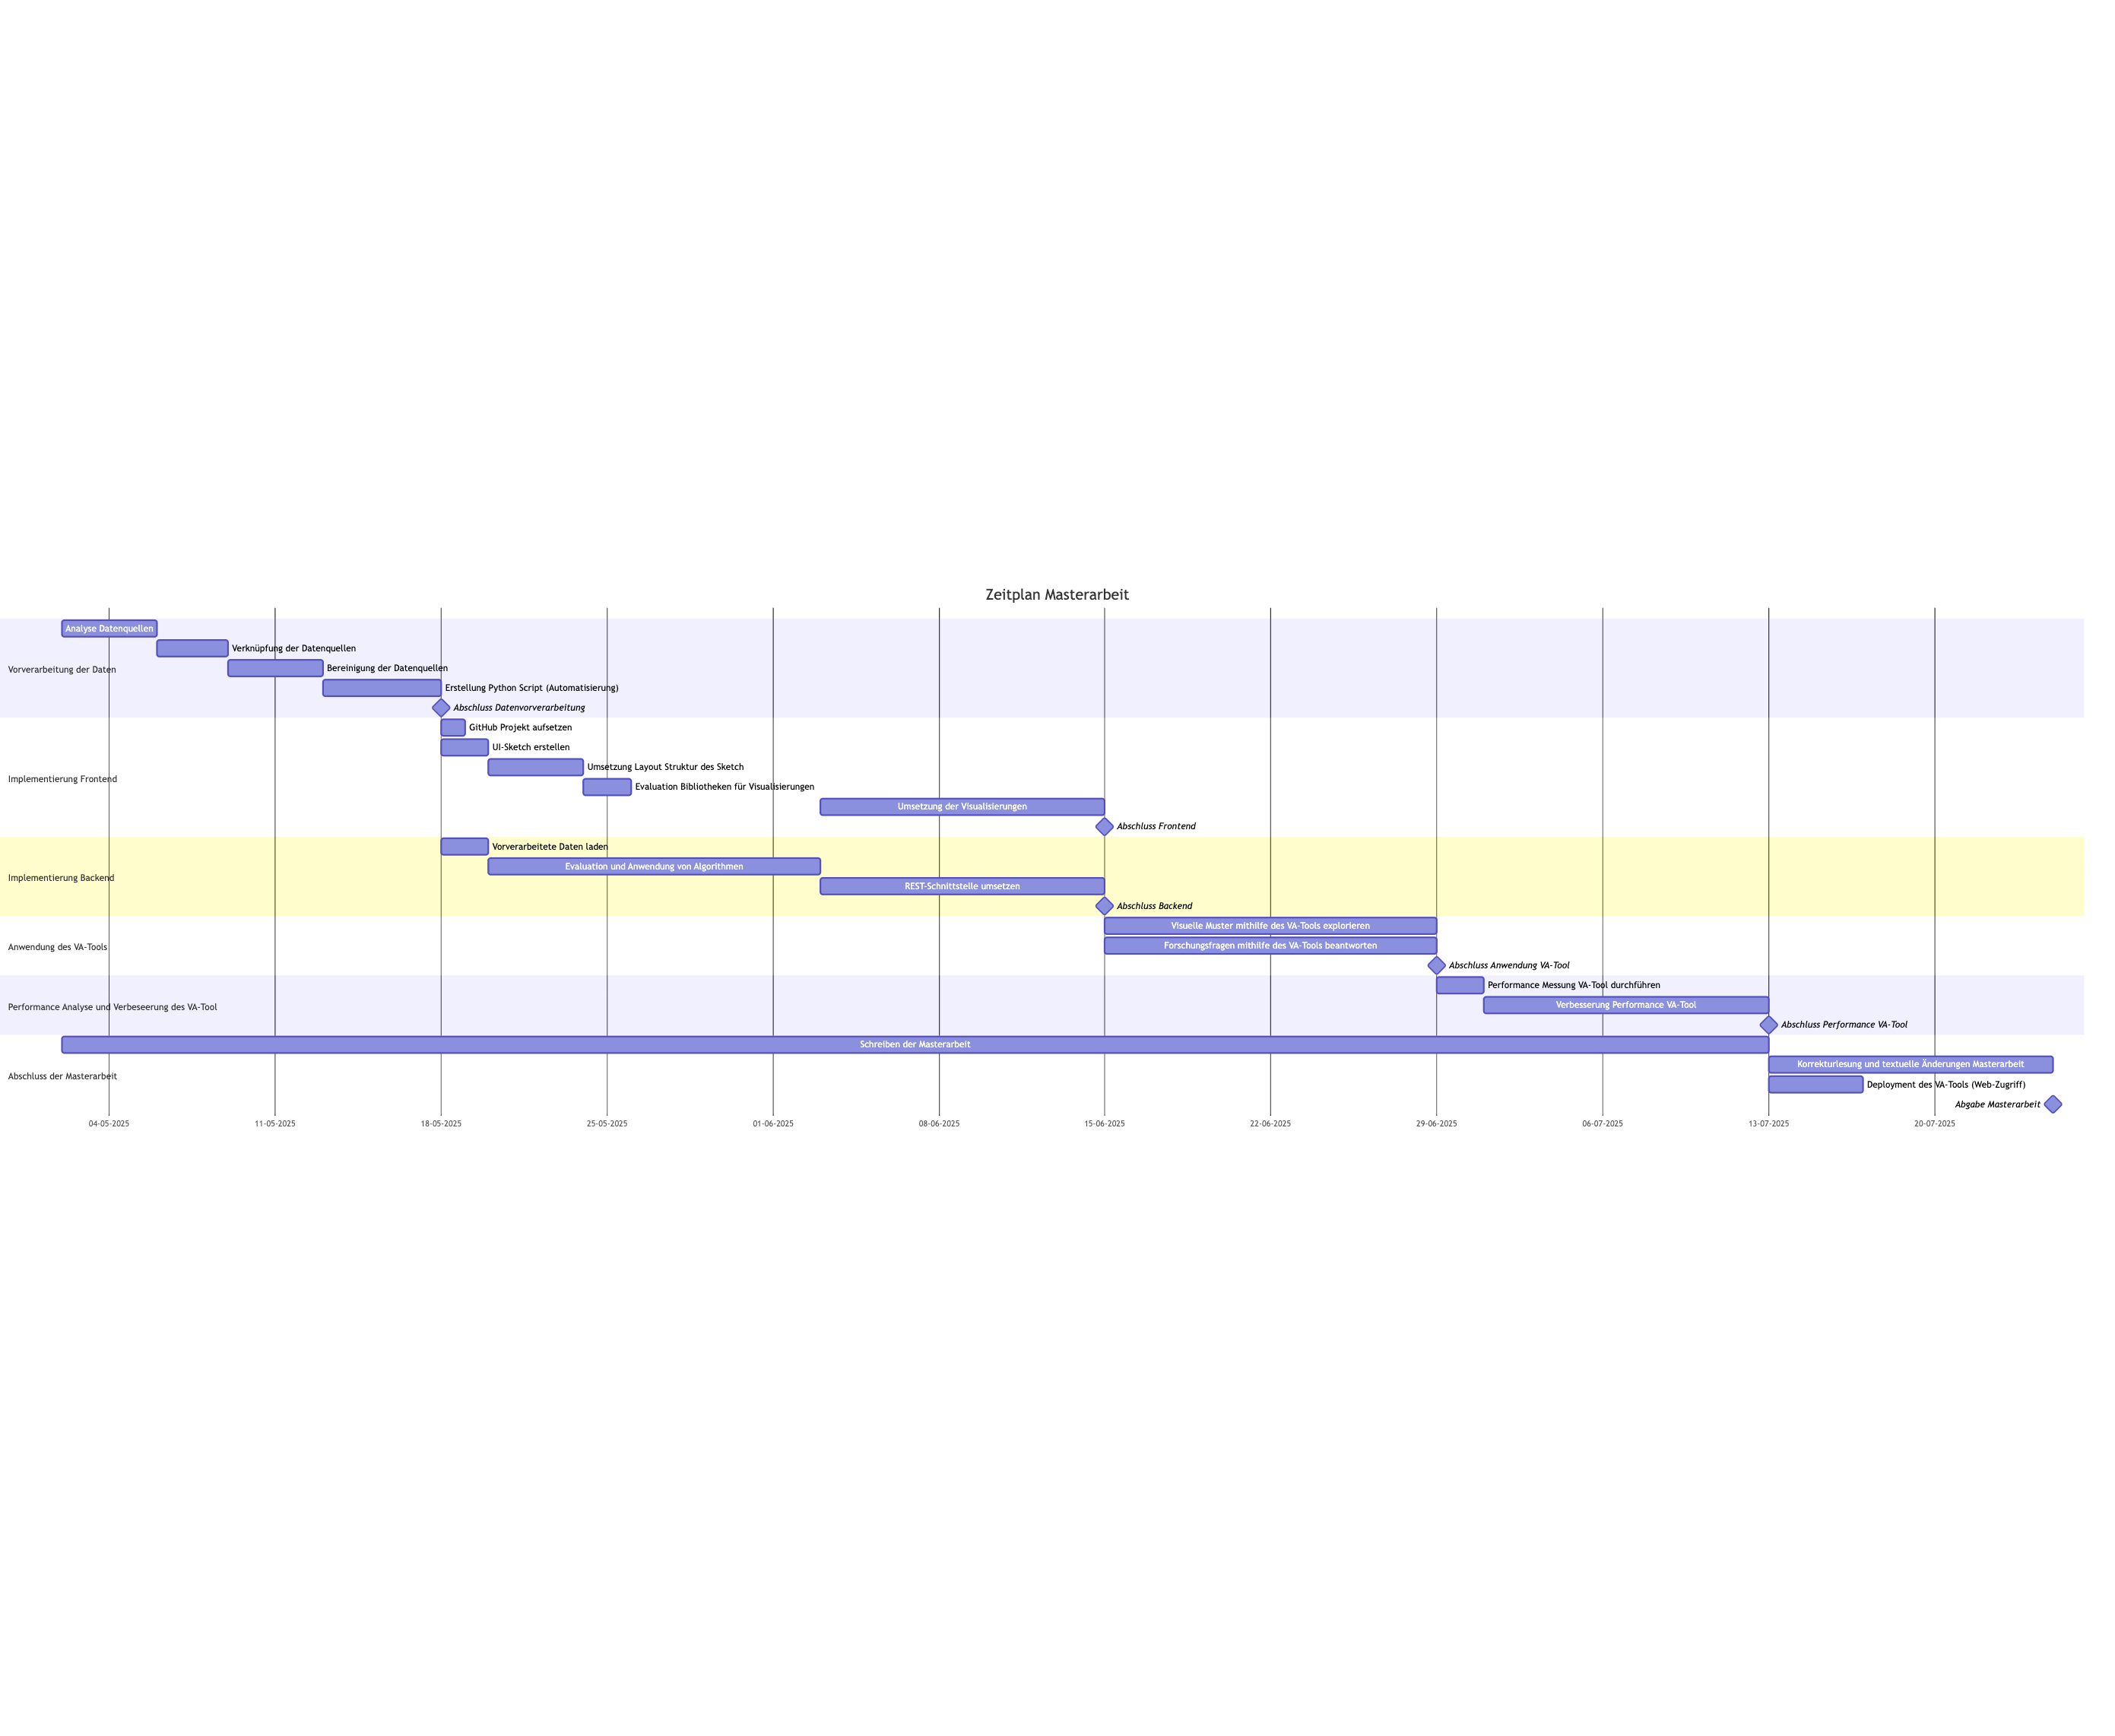
\includegraphics[width=1.0\linewidth, angle=90]{content/00_assets/meilensteine_gantt_diagram.png}
    \label{fig_zeitplan}
\end{figure}

\newpage

\section{Code zur Generierung des Zeitplans}
Der Zeitplan wurde mithilfe von Mermaid\footnote{\url{https://mermaid.js.org/}} erstellt. Hierzu wurde folgender Code genutzt:

\begin{lstlisting}
gantt
    title Zeitplan Masterarbeit
    dateFormat DD-MM-YYYY
    axisFormat %d-%m-%Y
    section Vorverarbeitung der Daten
        Analyse Datenquellen :analyse_datenformat, 02-05-2025, 4d
        Verknüpfung der Datenquellen :verknuepfung_datenquellen, after analyse_datenformat, 3d
        Bereinigung der Datenquellen :bereinigung_datenquellen, after verknuepfung_datenquellen, 4d
        Erstellung Python Script (Automatisierung) :vorverarbeitung_python_script, after bereinigung_datenquellen, until abschluss_datenvorverarbeitung
        Abschluss Datenvorverarbeitung :milestone, abschluss_datenvorverarbeitung, 18-05-2025, 0d 
    section Implementierung Frontend
        GitHub Projekt aufsetzen :github_projekt_aufsetzen, after abschluss_datenvorverarbeitung, 1d
        UI-Sketch erstellen :frontend_sketch, after abschluss_datenvorverarbeitung, 2d
        Umsetzung Layout Struktur des Sketch :frontend_layout, after frontend_sketch, 4d
        Evaluation Bibliotheken für Visualisierungen :frontend_framework_evaluation, after frontend_layout, 2d
        Umsetzung der Visualisierungen :frontend_umsetzung_visualisierungen, after backend_algorithmen, until abschluss_frontend
        Abschluss Frontend :milestone, abschluss_frontend, 15-06-2025, 0d
    section Implementierung Backend
        Vorverarbeitete Daten laden :backend_daten_laden, after abschluss_datenvorverarbeitung, 2d
        Evaluation und Anwendung von Algorithmen :backend_algorithmen, after backend_daten_laden, 14d
        REST-Schnittstelle umsetzen :backend_rest_schnittstelle, after backend_algorithmen, until abschluss_backend
        Abschluss Backend :milestone, abschluss_backend, 15-06-2025, 0d
    section Anwendung des VA-Tools
        Visuelle Muster mithilfe des VA-Tools explorieren :visuelle_muster_va_tool, after abschluss_backend, until abschluss_anwendung_va_tool
        Forschungsfragen mithilfe des VA-Tools beantworten :forschungsfragen_beantworten_va_tool, after abschluss_backend, until abschluss_anwendung_va_tool
        Abschluss Anwendung VA-Tool :milestone, abschluss_anwendung_va_tool, 29-06-2025, 0d
    section Performance Analyse und Verbeseerung des VA-Tool
        Performance Messung VA-Tool durchführen :performance_messung_va_tool, after abschluss_anwendung_va_tool, 2d
        Verbesserung Performance VA-Tool :performance_verbesserung_va_tool, after performance_messung_va_tool, until performance_verbesserung_va_tool_abschluss
        Abschluss Performance  VA-Tool :milestone, performance_verbesserung_va_tool_abschluss, 13-07-2025, 0d
    section Abschluss der Masterarbeit
        Schreiben der Masterarbeit :masterarbeit_schreiben, 02-05-2025, until masterarbeit_korrekturlesung
        Korrekturlesung und textuelle Änderungen Masterarbeit :masterarbeit_korrekturlesung, after performance_verbesserung_va_tool_abschluss, until abgabe_masterarbeit
        Deployment des VA-Tools (Web-Zugriff) :deployment_va_tool, after performance_verbesserung_va_tool_abschluss, 4d
        Abgabe Masterarbeit :milestone, abgabe_masterarbeit, 25-07-2025, 0d
\end{lstlisting}